%%%%%%%%%%%%%%%%%%%%%%%%%%%%%%%
% Template for bwHPC-Symposium 
% (compile with pdflatex)
%%%%%%%%%%%%%%%%%%%%%%%%%%%%%%%

%
% --- do NOT change anything here ---
%

\documentclass[fontsize=11pt,a4paper]{article}
\usepackage[T1]{fontenc}
\usepackage[utf8]{inputenc}
\usepackage[english]{babel}
\usepackage{graphicx}
\usepackage[a4paper]{geometry}
\geometry{outer=2.5cm, inner=2.5cm, top=3.5cm, bottom=3.5cm}
\usepackage{lmodern}
\usepackage{lineno}
\usepackage{color}
\newcommand{\red}[1]{\textcolor{red}{#1}}
\newcommand{\changed}[1]{{#1}}
% \newcommand*{\REVIEW}{} % comment this out in the final version of the document
\ifdefined\REVIEW
   \linenumbers
   \renewcommand{\changed}[1]{\textcolor{red}{#1}}
\fi

% switch font family to using sans-serif by default for everything (except mathematics)
\renewcommand{\familydefault}{\sfdefault}

%
% --- optional packages ---
%

%\usepackage{verbatim}
\usepackage{hyperref}
\usepackage{amsmath} 
\usepackage{amsfonts} 
\usepackage{amssymb}
\usepackage{xcolor}
\usepackage{listings}
\usepackage{siunitx}

%
% --- define some settings ---
%
\definecolor{beige}{RGB}{255, 240, 230}
\lstset{
    backgroundcolor=\color{beige},
    frame=single,
    keepspaces=true,
    captionpos=b,
}

\setlength\parindent{0pt}

%
% --- title and author ---
%

\title{cellular\_raza - Novel Flexibility in Design of Agent-Based Models in Cellular Systems}

\author{
    Jonas Pleyer, Christian Fleck\\\\
    Freiburg Center for Data Analysis, Modeling and AI\\
    University of Freiburg
}

%
% --- print date and title ---
%

\date{21.11.2024}
\begin{document}
\maketitle

%
% --- main contents starts here ---
%

\begin{abstract}
    This paper uses \texttt{cellular\_raza} to develop a model with cell-type specific interactions
    whereby cells self-assemble into regions of similar species which is also known as cell-sorting.
    We use this model to asses the parallelization performance of the numerical backend at the core
    of \texttt{cellular\_raza} and show that values of up to $p=97.78\pm0.14\%$ parallelizable code
    can be achieved, which indicates a high level of parallelizability.
\end{abstract}

% ##################################################################################################
\section{Introduction}\label{introduction}
% ##################################################################################################

\texttt{cellular\_raza} is a cellular agent-based modeling framework~\cite{Pleyer2023} which 
allows researchers to construct models from a clean slate.
In contrast to other agent-based modelling toolkits, it is free of assumptions about the underlying
cellular representation.
This enables researchers to build up complex models while retaining full control over every
parameter and behaviour introduced.

At the 9th bwHPC Symposium 2023, we presented a very compacted variety of applications and analytics
of \texttt{cellular\_raza}~\cite{PeaceOfPostersbwHPC}.
Here, we focus on the cell-sorting example which was also presented but has been refined since then.
We refer the interested reader to the documentation website
\href{https://cellular-raza.com}{cellular-raza.com} where one can find the full documentation,
remaining examples and information about the underlying assumptions and methods which we leveraged
in the development of \texttt{cellular\_raza}.

% ##################################################################################################
\section{Cell Sorting}
\label{sec:cell-sorting}
% ##################################################################################################

Cell Sorting is a naturally occuring phenomenon which drives many biological
processes~\cite{Steinberg1963,Graner1992}.
While the biological reality can be quite complex, it is rather simple to describe such
a system in its most basic form.
The underlying principle is that interactions between cells are specific with respect to their type.

\paragraph{Mathematical Description}
We assume that our cells are spherical objects which interact via force potentials.
The two positions of cells are $x_i,x_j$ and their distance is $r_{i,j}=||x_i-x_j||$.

\begin{align}
    \kappa_{i,j} &= \frac{r_{i,j}}{R_i + R_j}\\
    U_{i,j} &= V_0 \left(\frac{1}{3\kappa_{i,j}^3} - \frac{1}{\kappa_{i,j}}\right).
\end{align}

The values $R_i,R_j$ are the radii of the cells ($i\neq j$) interacting with each other.
For simplification, we can assume that they are identical $R_i=R_j=R$.
Furthermore, we assume that the equation of motion is given by

\begin{equation}
    \partial^2_t \vec{x}_i = \vec{F}_i - \lambda \partial_t \vec{x}_i
\end{equation}

where the first term is the usual force term $\vec{F}_i = - \sum_j\vec{\nabla} V_{i,j}$ obtained by
differentiating the given potential and the second term is a damping term which arises due to the
cells being immersed inside a viscuous fluid.
Note that we rescaled the units of our parameters in order to normalize our mass to $m=1$.
This means, every parameter can be expressed in units of length and time.

We can assume that interactions between cells are restricted to close ranges and thus enforce a
cutoff $\xi\geq R_i+R_j$ for the interaction where the resulting force is identical to zero.
We further assume that cells of different species do not attract each other but do repel.
To describe this behaviour, we set the potential to zero when $r>R_i+R_j$ (i.e., $\kappa_{i,j}>1$)
and both cells have distinct species type $s_i$.

\begin{equation}
    V_{i,j} =
    \begin{cases}
        0 &\text{ if } \kappa_{i,j}\geq\xi/(R_i+R_j)\\
        0 &\text{ if } s_i\neq s_j \text{ and } \kappa_{i,j}\geq 1\\
        U(\kappa_{i,j}) &\text{ else }
    \end{cases}.
\end{equation}

\paragraph{Parameters}
In total, we are left with only 4 cellular parameters to describe our system.
In order to fully specify the system, we also need to define the time for which we are solving, the
overall physical size and the initial number of agents which we put into the simulation.

\begin{table}
    \centering
    \begin{tabular}{l c c}
        Parameter & Symbol & Value\\
        \hline
        Cell Radius & $R_i$ & $\SI{6}{\micro\metre}$\\
        Potential Strength & $V_0$ & $\SI{2}{\micro\metre^2\per\minute^2}$\\
        Damping Constant & $\lambda$ & $\SI{2}{\per\minute}$\\
        Interaction Range & $\xi$ & $1.5 (R_i+R_j)=3R_i$\\
        \hline
        Time Stepsize & $\Delta t$ & $\SI{0.2}{\minute}$\\
        Time Steps & $N_t$ & $10'000$\\
        Domain Size & $L$ & $110\text{ µm}$\\
        Cells Species 1 & $N_{C,1}$ & $800$\\
        Cells Species 2 & $N_{C,2}$ & $800$\\
    \end{tabular}
    \caption{
        This table shows two sections containing parameters and other variables respectively which
        to fully specify and initialize the system.
        In total, 1600 cells with random initial positions and zero velocity were placed inside the
        domain.
    }
    \label{tab:cell-sorting-parameters}
\end{table}

\paragraph{Results}
Figure~\ref{fig:cell-sorting-results} shows the inital placement of the cells and their final state.
We can clearly see that the cells have assembled into connected regions of the same species.
The size of these regions depends on the interaction range and its strength.
In this example, we did not assume any stochastic motion of the cells.
It is to be noted that this assumption is not required by \texttt{cellular\_raza} but rather a
free choice of the model.
Depending on the desired complexity, users can substantially modify the cellular representation,
which is the main reason for the development of \texttt{cellular\_raza}.
We provide two additional
\href{https://github.com/jonaspleyer/cellular_raza/cellular_raza-examples/cell_sorting}{examples}
which implement mechanics with Brownian~\cite{Schlick2002} and
Langevin~\cite{Schlick2002,Pastor1994} dynamics but even more complex cellular representations are
possible as well (see eg. \href{https://cellular-raza.com/showcase/bacterial-rods}{bacterial-rods}).

\begin{figure}
    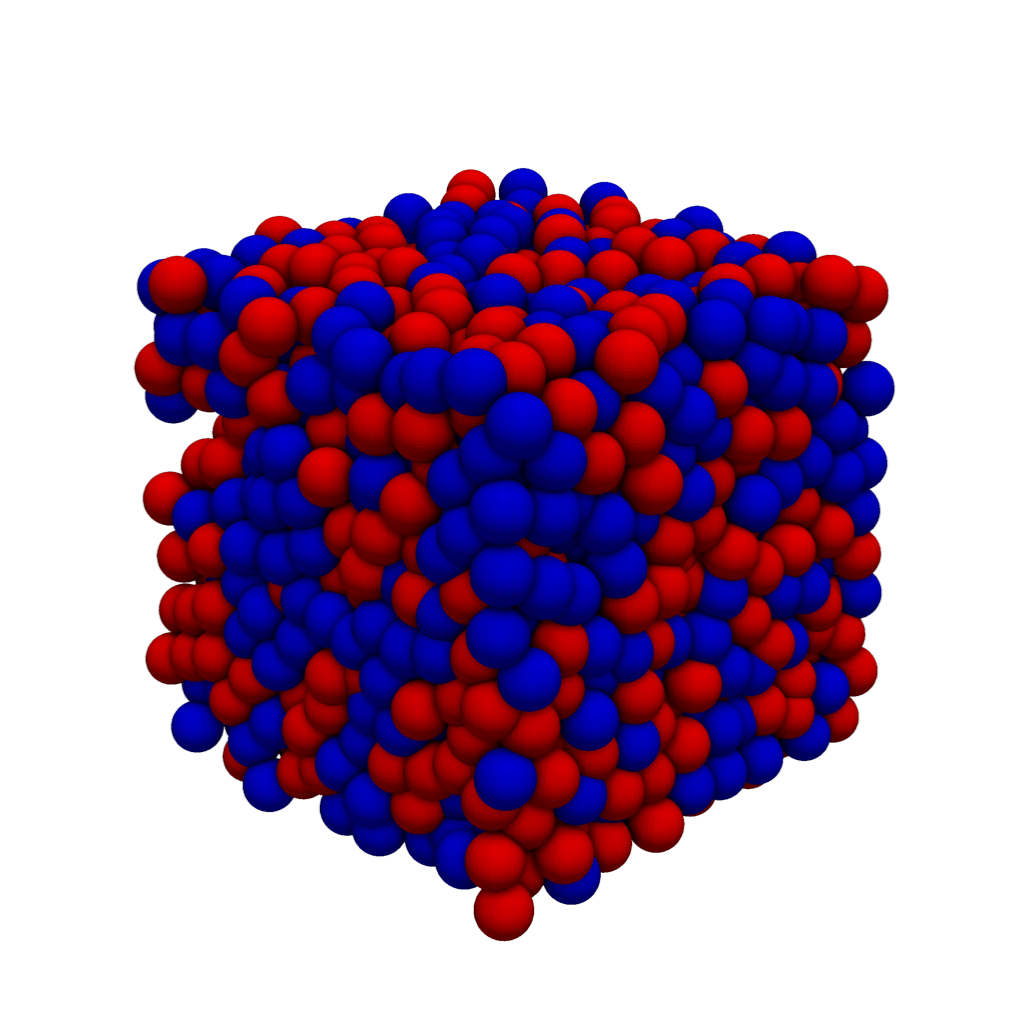
\includegraphics[width=0.5\textwidth]{figures/cell_sorting/0000000020.png}%
    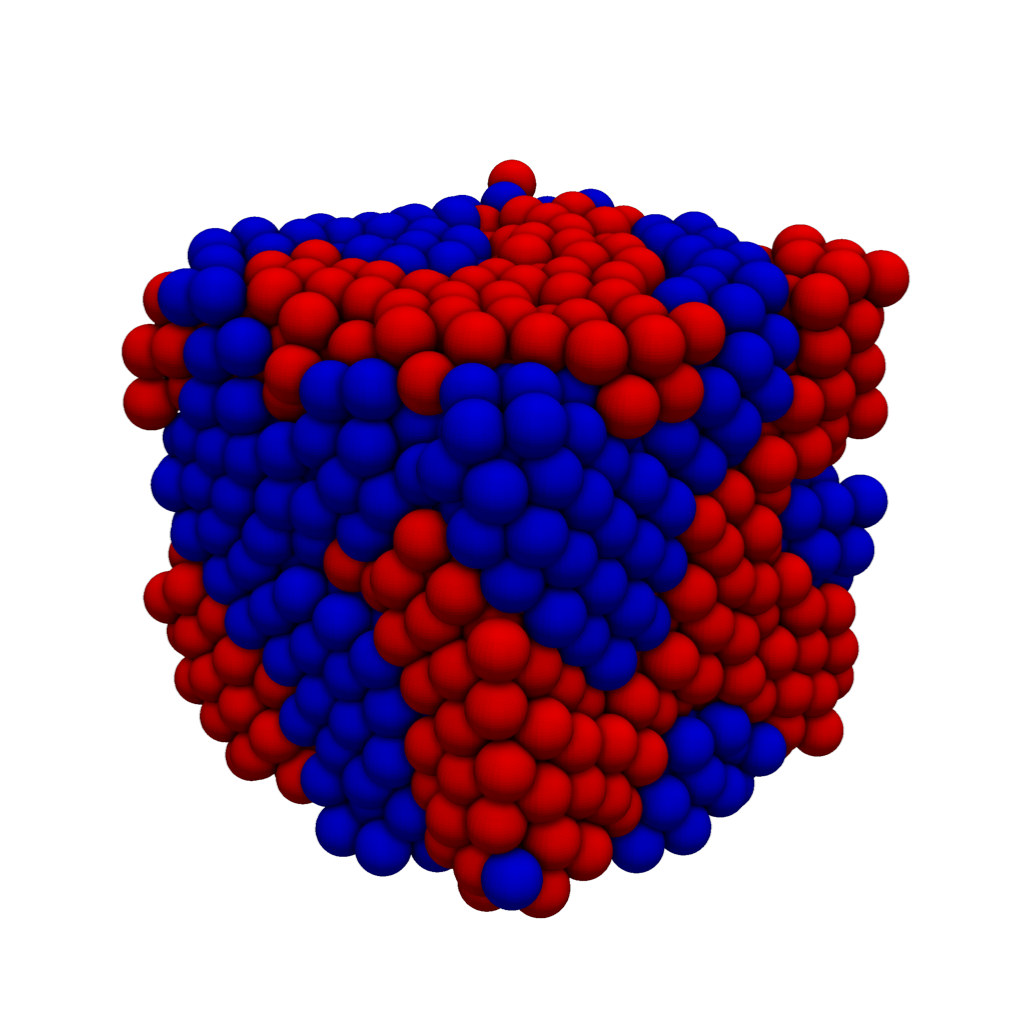
\includegraphics[width=0.5\textwidth]{figures/cell_sorting/0000010000.png}
    \caption{
        Cells are initially placed randomly inside the cuboid simulation domain.
        After the simulation has finished, the cells have assembled into connected regions of the
        same species.
    }
    \label{fig:cell-sorting-results}
\end{figure}

% ##################################################################################################
\section{Multithreading Performance (Amdahl's Law)}
% ##################################################################################################

\paragraph{Theory}
One measure of multithreaded performance is to calculate the possible theoretical speedup
given by Amdahl's law~\cite{Rodgers1985}.
It provides an estimate for the speedup and assumes that the workload can be split into a
parallelizable and non-parallelizable part which is quantified by $0\leq p \leq1$.
A higher value means that the contribution coming from non-parallelizable algorithms is lower.
The theoretical maximum $p=1$ means that all of the executed code is parallelizable.
Amdahl's law is given by

\begin{equation}
    T(n) = T_0\frac{1}{(1-p) + \frac{p}{n}}
    \label{eq:amdahls-law}
\end{equation}

where $T(n)$ describes the throughput which can be achieved given $n$ parallel threads and the
variable $p$ is the relative proportion of execution time which benefits from parallelization.
The total latency of a program can be determined via the inverse of the throughput.

\paragraph{Simulation Setup}
Measuring the performance of any simulation will be highly dependent on the specific cellular 
properties and complexity.
For this comparison, we chose the previously explained cell-sorting example which contains minimal
complexity compared to other examples (see
\href{https://cellular-raza.com/showcase}{cellular-raza.com/showcase}).
Any computational overhead which is intrinsic to \texttt{cellular\_raza} and not related to the
chosen example would thus be more likely to manifest itself in performance results.

In order to produce reproducible results and simplify this overall process, we provide the
\href{https://github.com/jonaspleyer/cellular_raza-benchmarks}{cellular\_raza-benchmarks} crate.
It is a command-line utility which can be used to run benchmarks with various configurations.

\begin{minipage}{\linewidth}\begin{lstlisting}[
    language=Bash,
    basicstyle=\ttfamily\footnotesize,
    caption={
        Usage of the benchmark CLI tool.
        We provide two benchmarks, one for increasing the number of agents and another for
        increasing the number of threads.
        The subcommands can be further customized and will automatically run the given simulation
        multiple times for the specified configurations.
    }
]
# cd cellular_raza-benchmarks
# cargo run -- -h
cellular_raza benchmarks

Usage: cell_sorting [OPTIONS] <NAME> [COMMAND]

Commands:
  threads   Thread scaling benchmark
  sim-size  Simulation Size scaling benchmark
  help      Print this message or the help of the given subcommand(s)

Arguments:
  <NAME>  Name of the current runs such as name of the device to be benchmarked

Options:
  -o, --output-directory <OUTPUT_DIRECTORY>
          Output directory of benchmark results [default: benchmark_results]
  -s, --sample-size <SAMPLE_SIZE>
          Number of samples to be generated for each measurement [default: 5]
      --no-save
          Do not save results. This takes priority against the overwrite settings
      --overwrite
          Overwrite existing results
      --no-output
          Disables output
  -h, --help
          Print help
  -V, --version
          Print version
\end{lstlisting}\end{minipage}

Results generated in this way are stored inside the \texttt{benchmark\_results} folder.
In addition, we provide a python script \texttt{plotting/cell\_sorting.py} to quickly visualize
the obtained results.

\paragraph{Hardware}
This benchmark was run on three distinct hardware configurations.
There exists a wide range of variables which could influence our measured runtime results.
However, we expect that the biggest effects are due to power-limits and variable frequency of the
central processing unit (CPU).
Both of these effects can be circumvented by choosing an artificially fixed frequency which is low
enough such that the total power limit of the CPU is never reached even when multiple cores are
under load.
While it is well known that other aspects such as cache-size and memory latency can have an impact
on absolute performance, they should however not introduce any significant deviations in terms of
relative performance scaling.

\begin{table}
    \centering
    \begin{tabular}{l c c c}
        CPU & Fixed Clockspeed & Memory Frequency & TDP\\
        \hline
        AMD Ryzen 3700X~\cite{AMDProductSpecifications} & $\SI{2200}{\mega\hertz}$
            & $\SI{3200}{\mega T\per\second}$ & $\SI{65}{\watt}$\\
        AMD Ryzen Threadripper 3960X~\cite{AMDProductSpecifications} & $\SI{2000}{\mega\hertz}$
            & $\SI{3200}{\mega T\per\second}$ & $\SI{280}{\watt}$\\
        Intel Core i7-12700H~\cite{Inteli712700H} & $\SI{2000}{\mega\hertz}$
            & $\SI{4800}{\mega T\per\second}$
            & $\SI{45}{\watt}$\\
    \end{tabular}
    \caption{List of tested hardware configurations.}
    \label{tab:hardware-configurations}
\end{table}

\paragraph{Results}

\begin{figure}
    \centering
    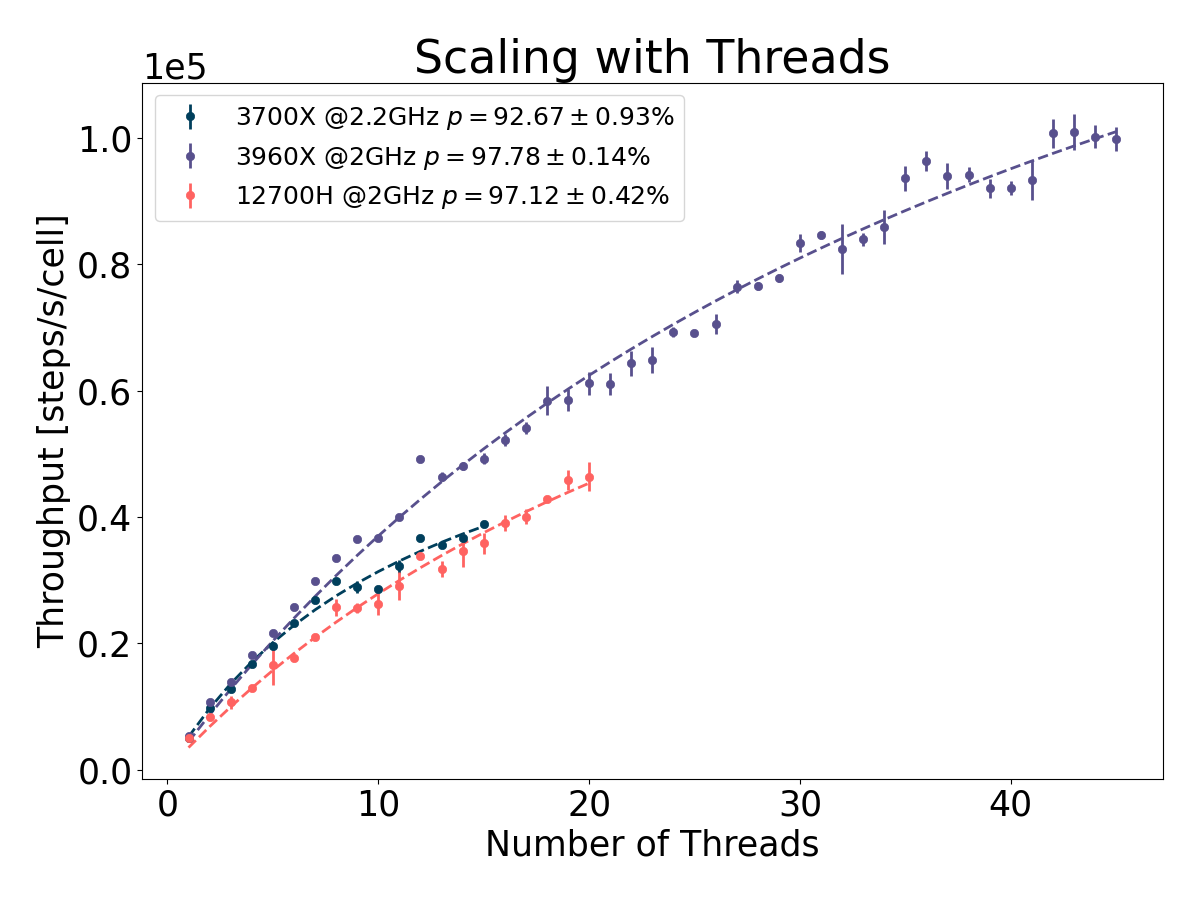
\includegraphics[width=0.8\textwidth]{figures/thread_scaling.png}
    \caption{Performance of the throughput $T(n)$ for increasing number of utilized threads $n$.}
    \label{fig:amdahls-law-fit}
\end{figure}

In figure~\ref{fig:amdahls-law-fit}, we fit Amdahl's law of equation~\ref{eq:amdahls-law} to our
measured datapoints and obtain the parameter $p$ from which the theoretical maximal speedup $S$ can
be calculated via

\begin{equation}
    \lim\limits_{n\rightarrow\infty} T(n) = S = \frac{1}{1-p}
    \label{eq:amdahls-law-maximum-speedup}
\end{equation}

The values for the maximum theoretical speedup are $S_\text{3700X}=13.64\pm1.73$,
$S_\text{3960X}=44.99\pm2.80$ and $S_\text{12700H}=34.74\pm5.05$.
Their uncertainty $\sigma(S)$ can be calculated via the standard gaussian propagation

\begin{equation}
    \sigma(S) = \frac{\sigma(p)}{(1-p)^2}
\end{equation}

where $\sigma(p)$ is the uncertainty of the parameter $p$ obtained via the fit in
figure~\ref{fig:amdahls-law-fit}.

\paragraph{Discussion}
The perfect score of a fully parallelizable system with $p=1$ is considered almost unobtainable
in a real-world scenario due to effects such as the workload of the underlying operating system
and physical constraints.
Our results showed that the measured value $p$ does also depend on the respective hardware.

In addition to hardware-related effects, we also expect a portion of $1-p$ of our simulation code
to be fundamentally not parallelizable.
This fraction can be made up of the initial setup of the simulation which necessarily has to start
single-threaded and can only extend to multiple workers once all respective
\href{https://cellular-raza.com/docs/cellular_raza_core/backend/chili/struct.SubDomainBox.html}
{subdomains} are generated
\href{https://cellular-raza.com/docs/cellular_raza_concepts/trait.Domain.html}{generated}.
Furthermore, ending the simulation not only frees resources which requires computation but also
locks the main routine until every individual thread has finished.
Even more importantly, all threads are currently using a shared barrier~\cite{GjengsetHurdles2018}
to sync with each other which means that even a single worker can block all others.
This limitation could be fixed in the future with improved versions \texttt{cellular\_raza} and is
only an implementation detail and not a fundamental drawback.

However, the total speedup $S$ is still very good for all configurations which can be directly
attributed to a good implementation and the core assumption of \texttt{cellular\_raza} that
\href{https://cellular-raza.com/guides/introduction/#local-rules}
{all interactions are strictly local} and subdomains are only interacting along their borders
without the need to construct long-ranging synchronization algorithms.

% ##################################################################################################
\section{Conclusions}\label{conclusions}
% ##################################################################################################

We showed along the example of cell-sorting how \texttt{cellular\_raza} can be used to model
cellular biological systems.
The modeling process is flexible due to the variety of cellular representations which are supported.
We chose to represent our cells with only 4 parameters, which specify the physical representation
and interaction of the cells.
The numerical results showed the expected behaviour of cells assembling into connected regions of
identical species.\\
Utilizing the cell-sorting simulation, we benchmarked the performance of the numerical backend.
We picked a simulation which is large enough to fully saturate all processors and gradually
increased the number of threads utilized.
The fractional amount of parallelizable code was determined by fitting the values of runtime to
Amdahl's law.
It reached values up to $p=97.78\%$ for a workstation setup which indicates a well-parallelizable
implementation.

% ##################################################################################################
\section{Acknowledgements} 
% ##################################################################################################

The author(s) declare that financial support was received for the research, authorship, and/or
publication of this article.
JP and CF received funding from FET-Open research and innovation actions grant
under the European Union’s Horizon 2020 (CyGenTiG; grant agreement 801041).

\bibliographystyle{IEEEtran}
\bibliography{references}

\end{document}
